\section{Merkmale modellieren}
\label{sec:Kap-4.2}

Merkmale von Realwelt-Objekten, zum Beispiel die Fellfarbe bei Katzen, definiert man in der objektorientierten Softwareentwicklung in den Klassen. Dafür verfügen die Klassen über sogenannte \textit{Attribute}.
\marginline{Attribute}

\vspace{2mm} %%% für Druck

\begin{figure}[h!]
	\centering
	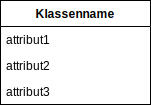
\includegraphics{Bilder/Kapitel-4/darstellung_klasse_mit_drei_attributen.pdf}
	\caption[Die UML-Darstellung einer Klasse]{Die UML-Darstellung einer Klasse mit Angabe des Namens der \mbox{Klasse} und drei Attributen}
	\label{fig:darstellung_klasse_mit_drei_attributen}
\end{figure}

In der UML-Darstellung wird das Rechteck der Klasse durch eine Linie horizontal unterteilt. Oberhalb der Linie steht der schon bekannte Name der Klasse, unterhalb der Linie werden die Attribute, untereinander und linksbündig gesetzt, aufgeführt. Jedes (spätere) Objekt, das nach den Vorgaben der Klasse modelliert wird – man sagt verkürzend: „Jedes Objekt der Klasse“ – verfügt über genau die Attribute, die die Klasse definiert. Die Werte der Attribute, also die Ausprägung der Merkmale, sind dabei jedoch spezifisch pro Objekt.

Wir wechseln von Katzen zu Autos! Abbildung~\ref{fig:klasse_auto_mit_zwei_attributen} zeigt eine Klasse \sttpUMLText{Auto} mit den zwei Attributen \sttpUMLText{modell} und \sttpUMLText{farbe}.

\begin{figure}[h!]
	\centering
	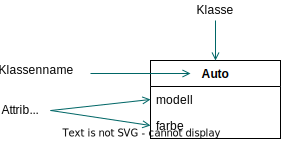
\includegraphics{Bilder/Kapitel-4/klasse_auto_mit_zwei_attributen.pdf}
	\caption{Eine Klasse \sttpUMLText{Auto} mit zwei Attributen}
	\label{fig:klasse_auto_mit_zwei_attributen}
\end{figure}

Abbildung~\ref{fig:drei_mal_klasse_auto_plus_klasse_hugoauto} oben zeigt mit \sttpUMLText{ellensAuto}, \sttpUMLText{heikesAuto} und \sttpUMLText{marvinsAuto} drei Objekte, die die von der Klasse \sttpUMLText{Auto} definierten Merkmale (Vorhandensein der Eigenschaften Modell und Farbe) erfüllen und damit Objekte der Klasse \sttpUMLText{Auto} sind. Die von der Klasse vorgegebenen Attribute sind bei den Objekten mit konkreten Werten belegt: Für das Attribut \sttpUMLText{modell} finden wir hier die Werte Toyota Yaris und VW Golf, für das Attribut \sttpUMLText{farbe} die Werte stahlblau, weiß und rot. Wie hier bei dem \sttpUMLText{modell}-Attribut von \sttpUMLText{ellensAuto} und \sttpUMLText{heikesAuto} können die Werte -- man sagt auch synonym: Wertebelegungen
\marginline{Werte\-belegungen}
-- von Attributen bei unterschiedlichen Objekten auch übereinstimmen. Wenn zwei Objekte derselben Klasse in \textbf{allen} \mbox{Wertebelegungen} der Attribute übereinstimmen, also zum Beispiel Heikes Toyota Yaris auch stahlblau wäre wie der von Ellen, nennt man dies in der Objektorientierung zustandsgleiche Objekte.

\begin{figure}[h!]
	\centering
	\includegraphics{Bilder/Kapitel-4/klasse_auto.pdf}
	\caption[Drei Objekte der Klasse \sttpUMLText{Auto}]{Drei Objekte der Klasse \sttpUMLText{Auto} (oben) und ein Objekt mit Namen \sttpUMLText{hugosAuto}, das kein Objekt der Klasse Auto aus Abbildung~\ref{fig:klasse_auto_mit_zwei_attributen} ist (unten)}
	\label{fig:drei_mal_klasse_auto_plus_klasse_hugoauto}
\end{figure}

Abbildung~\ref{fig:drei_mal_klasse_auto_plus_klasse_hugoauto} unten
\marginline{der Unterschied zwischen Realwelt-Objekten und modellierten Objekten}
zeigt ein Objekt mit Namen \sttpUMLText{hugosAuto}, das im Gegensatz zu den drei anderen Objekten kein Objekt der in Abbildung~\ref{fig:klasse_auto_mit_zwei_attributen} modellierten Klasse \sttpUMLText{Auto} ist, da es über ein Attribut \sttpUMLText{baujahr} verfügt, das die in Abbildung~\ref{fig:klasse_auto_mit_zwei_attributen} dargestellte Auto-Klasse nicht kennt. An dieser Stelle müssen Sie sich noch einmal den Unterschied zwischen Realwelt-Objekten und den für Softwareengineering-Zwecke modellierten Objekten vergegenwärtigen: Das Realwelt-Auto von Hugo ist sicher genau wie die Autos von Ellen, Heike und Marvin ein Auto. Und die Realwelt-Autos der drei letzteren Personen haben auch genau wie Hugos Auto ein Baujahr. Die in Abbildung~\ref{fig:klasse_auto_mit_zwei_attributen} für einen (hier unbekannten) Zweck im Rahmen des Softwareengineering modellierte Klasse Auto abstrahiert von allen Eigenschaften von Realwelt-Autos, die für den Modellierungszweck nicht relevant sind. Und in diesem Beispiel betrifft das eben auch das Merkmal Baujahr. \textbf{Modellierte} Objekte vom Typ Auto besitzen hier daher kein Attribut \sttpUMLText{baujahr}, auch wenn für ihre Realweltentsprechungen ein Baujahr existiert.

An dem Auto-Baujahr-Beispiel zeigt sich ein weiterer praktischer Verwendungszweck von Objektdiagrammen. In  Diskussionen über die relevanten Strukturen der Domäne zwischen Softwareentwicklungsteam und Kunden kann es für die Kunden schwierig sein, die ihnen bekannte Ebene der Realwelt-Objekte mit der Ebene der deutlich abstrakteren Klassen zusammenzubringen. Hier kann es helfen, statt Klassen zunächst konkrete (Beispiel)Objekte und ihre Eigenschaften zu modellieren und erst anschließend auf dieser Grundlage die benötigten Klassen zu entwerfen.